% Part 2 chapter carrying "Three-Way Mass Discrepancy in Galaxy Clusters as a Test of mu < 1, Sigma = 1: eROSITA X-ray, Planck SZ, and DES Weak
% Lensing" (25 Feb 2026) in its order. Read in full 2026-10-02 (PDF text 296 lines in this extraction, 304 in the check file's; every
% line read). Numbers: docs/verification/scripts/verify_obs_chapters.py (section E). Check: docs/verification/observations/THREE_WAY_CLUSTER_CHECK.md;
% errata TW1-TW6. Level 1 form only; the test is ON HOLD until the implementation form is settled (author, 2026-10-02).
\chapter{Three cluster masses}\label{ch:threeway}

\section*{The place}
The same clusters as Chapter~\ref{ch:lensdyn}, read three ways: by the X-ray gas held in hydrostatic equilibrium, by the Sunyaev--Zeldovich (SZ)
distortion that the hot electrons imprint on the CMB, and by the weak lensing of background galaxies. The first two answer to the potential that
matter feels; the third to the potential that light feels. This chapter states what the informational term predicts for the three, in the one
form in which it predicts a difference, and what remains open.

\section{Three estimators}
\begin{itemize}
\item \emph{X-ray hydrostatic mass.} The temperature and density profiles of the gas give the pressure gradient that balances the gravitational
acceleration the gas feels.
\item \emph{SZ mass.} The SZ signal $Y$ is converted to mass through a $Y$--$M$ scaling relation calibrated on hydrostatic X-ray masses. It inherits
whatever the X-ray masses carry.
\item \emph{Weak-lensing mass.} The shear of background galaxies measures the lensing potential $\Phi+\Psi$.
\end{itemize}

\section{The ratio in the Level 1 form}
In the Level~1 form the gas feels $\mu$ times the true acceleration, so $M_{\rm hydro}=\mu M_{\rm true}$, $M_{\rm SZ}\approx M_{\rm hydro}$ through the
calibration, and $M_{\rm lens}=\Sigma M_{\rm true}=M_{\rm true}$. The lensing-to-hydrostatic ratio is
\begin{equation}
R(z)\equiv\frac{M_{\rm lens}}{M_{\rm hydro}}=\frac{1}{\mu(z)},\qquad\mu(a)=\frac{H^2_{\Lambda\rm CDM}(a)}{H^2_{\Lambda\rm CDM}(a)+\beta_mE(a)H_0^2},
\label{eq:tw_R}\end{equation}
the curve of Eq.~\eqref{eq:ld_ratio}. \calc
\begin{center}\small\begin{tabular}{lcccccccccc}\toprule
$z$ & 0 & 0.1 & 0.2 & 0.3 & 0.4 & 0.5 & 0.7 & 1.0 & 1.5 & 2.0\\\midrule
$\mu$ & 0.8638 & 0.8856 & 0.9050 & 0.9218 & 0.9362 & 0.9482 & 0.9661 & 0.9822 & 0.9938 & 0.9977\\
$R$ & 1.158 & 1.129 & 1.105 & 1.085 & 1.068 & 1.055 & 1.035 & 1.018 & 1.006 & 1.002\\\bottomrule
\end{tabular}\end{center}
At the redshifts of eROSITA samples ($z\approx0.2$--$0.4$) the gravitational part of the ratio is $1.07$--$1.10$. \calc
\begin{figure}[htbp]\centering
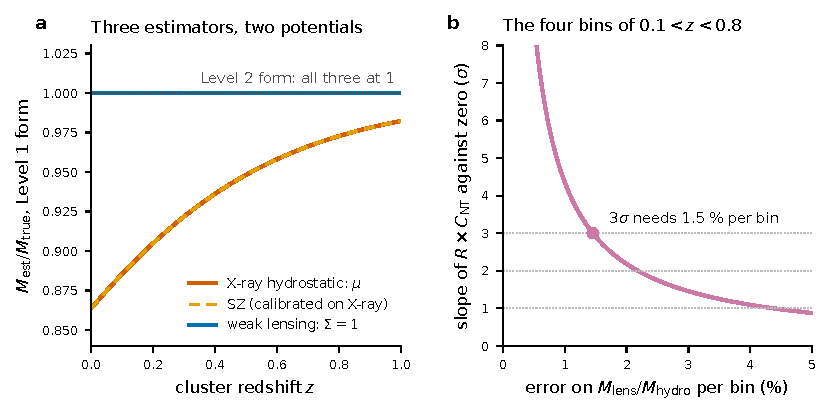
\includegraphics[width=\textwidth]{figures/part2/fig_threeway_estimators.pdf}
\caption[Three cluster mass estimators and the slope test]{(a) The three estimators over the true mass in the Level~1 form: the X-ray hydrostatic mass follows $\mu(z)$, the SZ mass follows it through the $Y$--$M$ calibration, and the weak-lensing mass follows $\Sigma=1$; in the Level~2 form all three are 1. \calc\ (b) The significance of a non-zero slope of $R\times C_{\rm NT}$ fitted as a straight line over the four bin centres (slope $-0.152$), against the fractional error per bin (equal errors): $3\sigma$ needs 1.5\,\% per bin. $C_{\rm NT}$ is the illustrative form. \calc\ \openprob}\label{fig:threeway_estimators}
\end{figure}

\section{The slope}
\calc\ The redshift slope is negative: $dR/dz=-0.183$ at $z=0.3$. Non-thermal pressure from turbulence and bulk motion gives the opposite sign,
because higher-redshift clusters are less relaxed~\cite{Nelson2014,ShiKomatsu2014}. For illustration take a factor
$C_{\rm NT}=1+0.20(1+z)^{0.2}$, whose slope is $+0.027$ to $+0.036$ over $0.15<z<0.65$; the form is assumed, not fitted to the simulations. With it, the two effects combine as
\begin{center}\small\begin{tabular}{lcccc}\toprule
Bin & centre & $R$ (Level~1) & $C_{\rm NT}$ & $R\times C_{\rm NT}$\\\midrule
$0.1<z<0.2$ & 0.150 & 1.117 & 1.206 & 1.346\\
$0.2<z<0.3$ & 0.250 & 1.094 & 1.209 & 1.323\\
$0.3<z<0.5$ & 0.400 & 1.068 & 1.214 & 1.297\\
$0.5<z<0.8$ & 0.650 & 1.039 & 1.221 & 1.269\\\bottomrule
\end{tabular}\end{center}
The total falls slowly with redshift because the gravitational part falls faster than the non-thermal part rises. The discriminant is the sign of the
slope in a sample measured one way throughout, not the size of the offset, which hydrostatic bias alone can supply. \calc
\begin{figure}[htbp]\centering
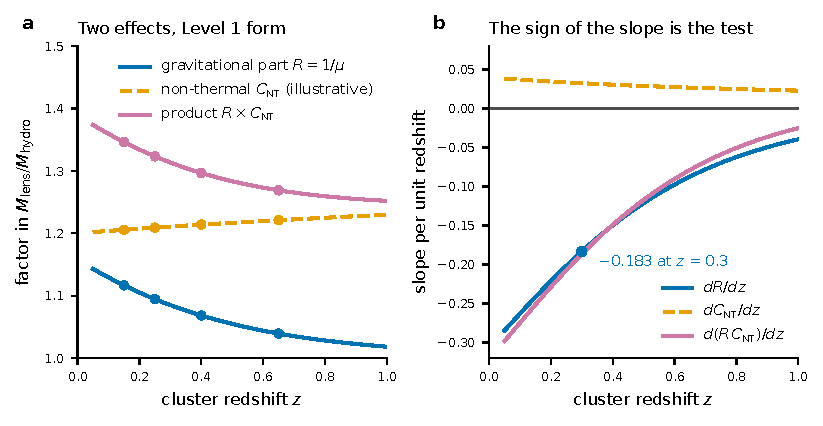
\includegraphics[width=\textwidth]{figures/part2/fig_threeway_slope.pdf}
\caption[The gravitational and non-thermal parts of the lensing-to-hydrostatic ratio]{Level~1 form. (a) The gravitational part $R=1/\mu$, the non-thermal factor $C_{\rm NT}=1+0.20(1+z)^{0.2}$ (illustrative form; normalisation and index still to be traced to simulations) and their product, with the four bin centres. (b) Their redshift slopes: $dR/dz=-0.183$ at $z=0.3$ against $dC_{\rm NT}/dz=+0.027$ to $+0.036$ over the bin centres; the product falls. In the Level~2 form $R=1$. Equations of \texttt{docs/verification/scripts/\allowbreak{}verify\_obs\_chapters.py}, section E. \calc\ \openprob}\label{fig:threeway_slope}
\end{figure}

\section{The SZ-to-X-ray ratio is not a test}
$M_{\rm SZ}/M_{\rm hydro}\approx1$ holds because the $Y$--$M$ relation is calibrated on hydrostatic masses. It holds in any theory of gravity, so it
cannot test the sector split, and it is not counted as a result here. The eROSITA cluster catalogue~\cite{Bulbul2024} provides the X-ray side of the
cross-match.

\section{The form of the term}
Equation~\eqref{eq:tw_R} needs $\mu$ in the Poisson equation for $\Psi$, the Level~1 effective-coupling form. In the Level~2 form the term
is a matter-sector expansion rate in the perturbation equations and the photon-sector equations and potentials are standard
(Chapter~\ref{ch:level2}); the potential then obeys the standard Poisson equation, gas in hydrostatic equilibrium feels the true acceleration, and
$R=1$: lensing--gas offsets follow the same collisionless dynamics as in $\Lambda$CDM, and differences enter only through the growth history. Which
form applies inside virialised clusters, and whether a linear $\mu$ applies there at all, is not derived. No comparison with published ratios is
made, and no forecast significance is quoted. \openprob

\section{What would test it}
\prediction\ In the Level~1 form: a cross-matched sample (eROSITA X-ray, Planck or ground-based SZ, Euclid or DES lensing) binned in redshift, one mass
method per estimator throughout, gives $R(z)$ falling with redshift as Eq.~\eqref{eq:tw_R} on top of a non-thermal part that rises. Falsified (in this
form) by a slope of zero or of positive sign after the non-thermal part is modelled from simulations. In the Level~2 form the prediction is $R=1$ apart
from astrophysics, and the clusters test only the growth history, through their abundance.

\section{Status}
\begin{center}\small\begin{tabularx}{\linewidth}{>{\raggedright\arraybackslash}Xl}\toprule
Result & Label\\\midrule
$R(z)=1/\mu(z)$ and its slope, Level~1 form & \calc\\
Sign of $dR/dz$ as the test & \prediction\ (Level~1 form)\\
Non-thermal factor $C_{\rm NT}$ (illustrative, assumed form) & \openprob\\
$M_{\rm SZ}/M_{\rm hydro}\approx1$ & \calibrated\ (not a test)\\
Implementation form inside clusters & \openprob\\\bottomrule
\end{tabularx}\end{center}
